\documentclass{beamer}
\mode<presentation>
{
\usepackage{dis-template}
}
\usepackage{listings}
\usepackage{hyperref}

\graphicspath{{slides/}} % TODO: eliminate this hack, necessary because scons builds at repository root

%---------------------------------------------------------------------
\titlepageinit{6}{Velocity Control}{25 \& 26 Feb 2015 (Week 6)}
%---------------------------------------------------------------------
\begin{document}
%---------------------------------------------------------------------
\begin{frame}
\titlepage

\setcounter{tocdepth}{1}
\tableofcontents
\end{frame}

%
% THIS IS INCOMPLETE. Obviously.
% The planned format doesn't seem to be conducive to slides either,
% as diagrams weren't ready (or really, necessary).
% Instead, notes are in docs/
%
% This may be updated one day with amazing ideas and diagrams.
%

% LAB PREPARATION
% Setup reference car demo

%---------------------------------------------------------------------
\section{Velocity Sensing} % [?? mins]
%---------------------------------------------------------------------
\begin{frame}
\centering \huge Velocity Sensing
\end{frame}

%---------------------------------------------------------------------
\subsection{Basics}

\begin{frame}
\frametitle{Brainstorm!}
\centering
What are some ways to sense velocity? \\
{\tiny pros and cons of your methods?}
\end{frame}

%---------------------------------------------------------------------
\subsection{Simple Encoder}

\begin{frame}
\frametitle{Optical Encoders}
\begin{columns}[t]
\column{0.646\textwidth}
Optical encoders...
\begin{itemize}
  \item Detects when sensor lit up
  \item Reflective sensor: light up codewheel, sensor detects reflection
  \item Photointerruptors: direct light beam from transmittor to detector, interrupt by object
  \item Simple designs vulnerable to ambient light
\end{itemize}

\hfill \\
Hamamatsu S6986...
\begin{itemize}
  \item High-pass filter and LED modulation for background light rejection
  \item Open-collector output
\end{itemize}

\column{0.323\textwidth}
\begin{figure}
  \centering
  % TODO: interruptor and reflective sensor OR Hamamatsu block diagram
  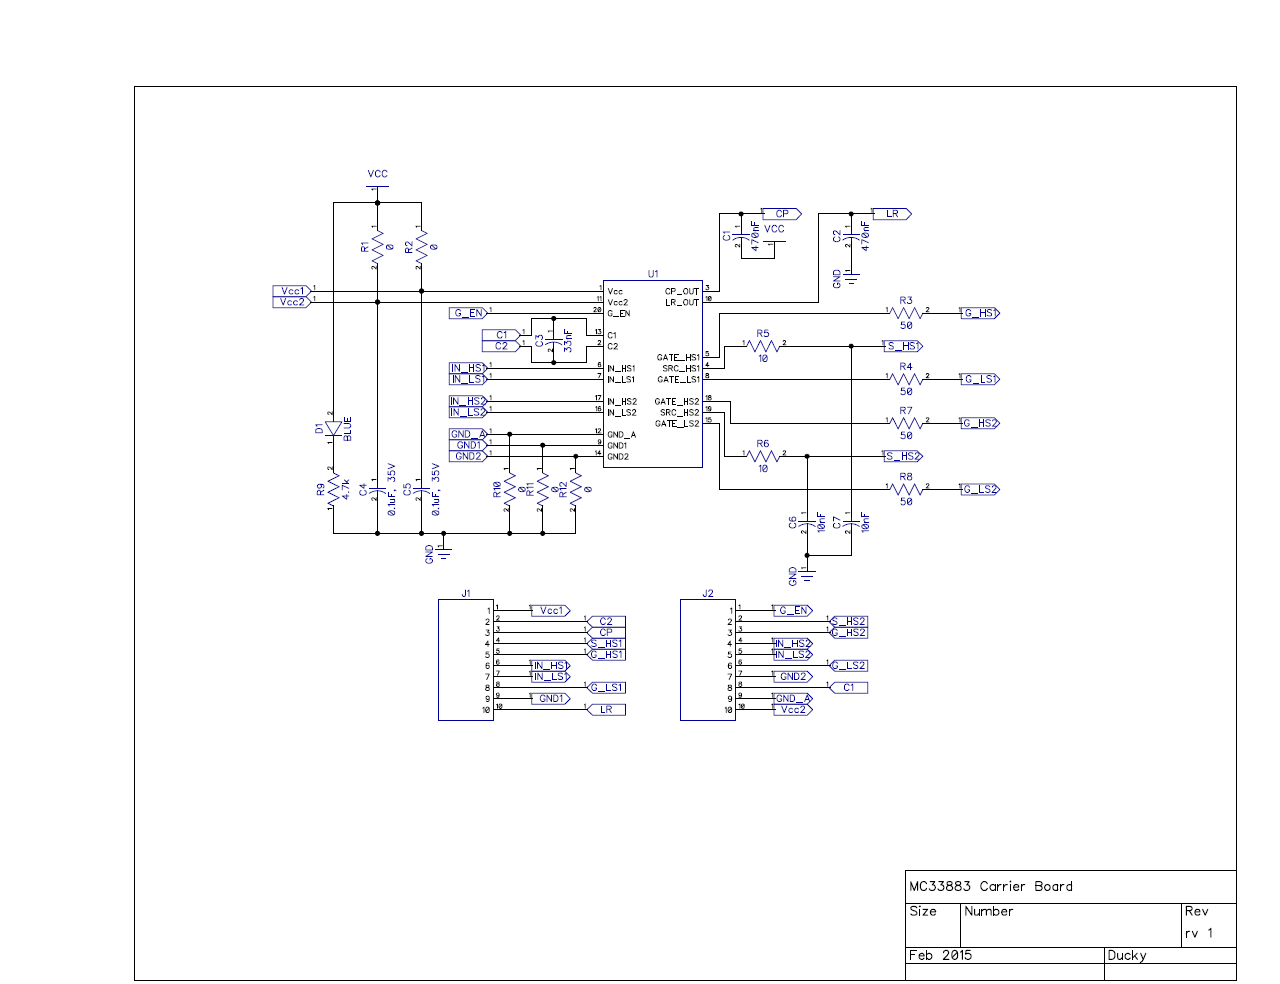
\includegraphics[width=1.0\columnwidth]{images-dis5/mc33883-schematic} \\
  Hopefully a fairly readable schematic
\end{figure}
\end{columns}
\end{frame}


\begin{frame}
\frametitle{Software Techniques}
\begin{columns}[t]
\column{0.646\textwidth}
Two simple ways to measure speed: \\
\hfill \\
Pulse width measurement
\begin{itemize}
  \item Measure width between transitions
\end{itemize} 

\hfill \\
Pulse counting
\begin{itemize}
  \item Count number of transitions in timespan
\end{itemize}

\hfill \\
Advantages and disadvantages of both?

\column{0.323\textwidth}
\begin{figure}
  \centering
  % TODO: quick illustration
  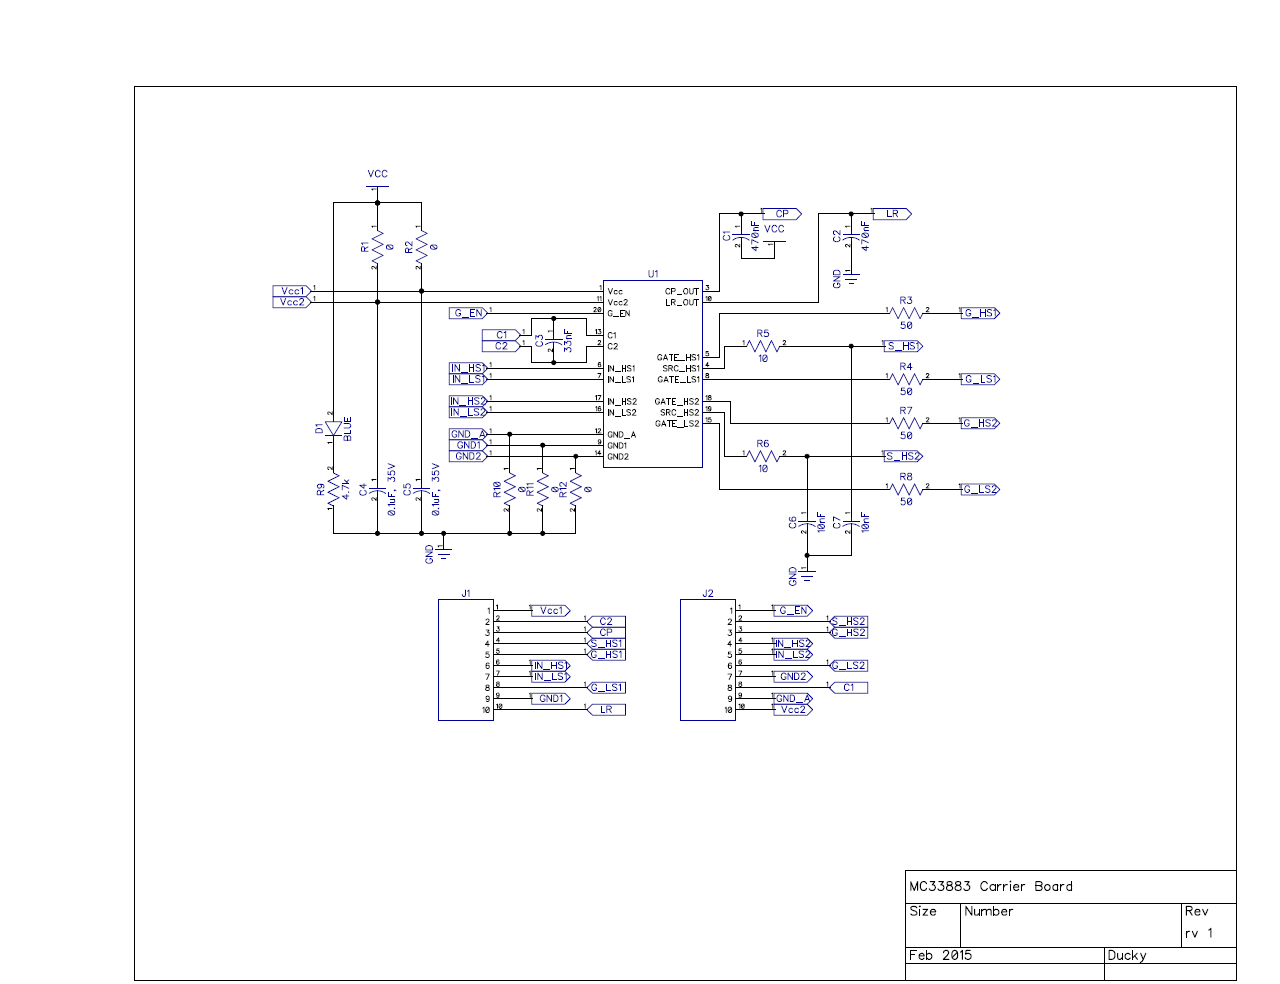
\includegraphics[width=1.0\columnwidth]{images-dis5/mc33883-schematic} \\
  Hopefully a fairly readable schematic
\end{figure}
\end{columns}
\end{frame}

\begin{frame}
\frametitle{Live Demo!}
\centering
Low speed demo \\
{\tiny see blinking LEDs!} \\
\hfill \\
High speed demo \\
{\tiny what waveforms should you expect to see?} \\
\hfill \\
Issues \\
{\tiny skipped pulses, inconsistent pulse lengths} \\
\end{frame}

%---------------------------------------------------------------------
\subsection{Issues}

\begin{frame}
\frametitle{Uh-oh!}
\centering
What are some ways to deal with inconsistent pulse sizing / other issues? \\
{\tiny pros and cons of your methods?}
\end{frame}

\begin{frame}
\frametitle{Moving Average Filter}
\begin{columns}[t]
\column{0.646\textwidth}
\begin{itemize}
  \item Average pulse widths over a entire revolution
\end{itemize}

\column{0.323\textwidth}
\begin{figure}
  \centering
  % TODO: quick illustration
  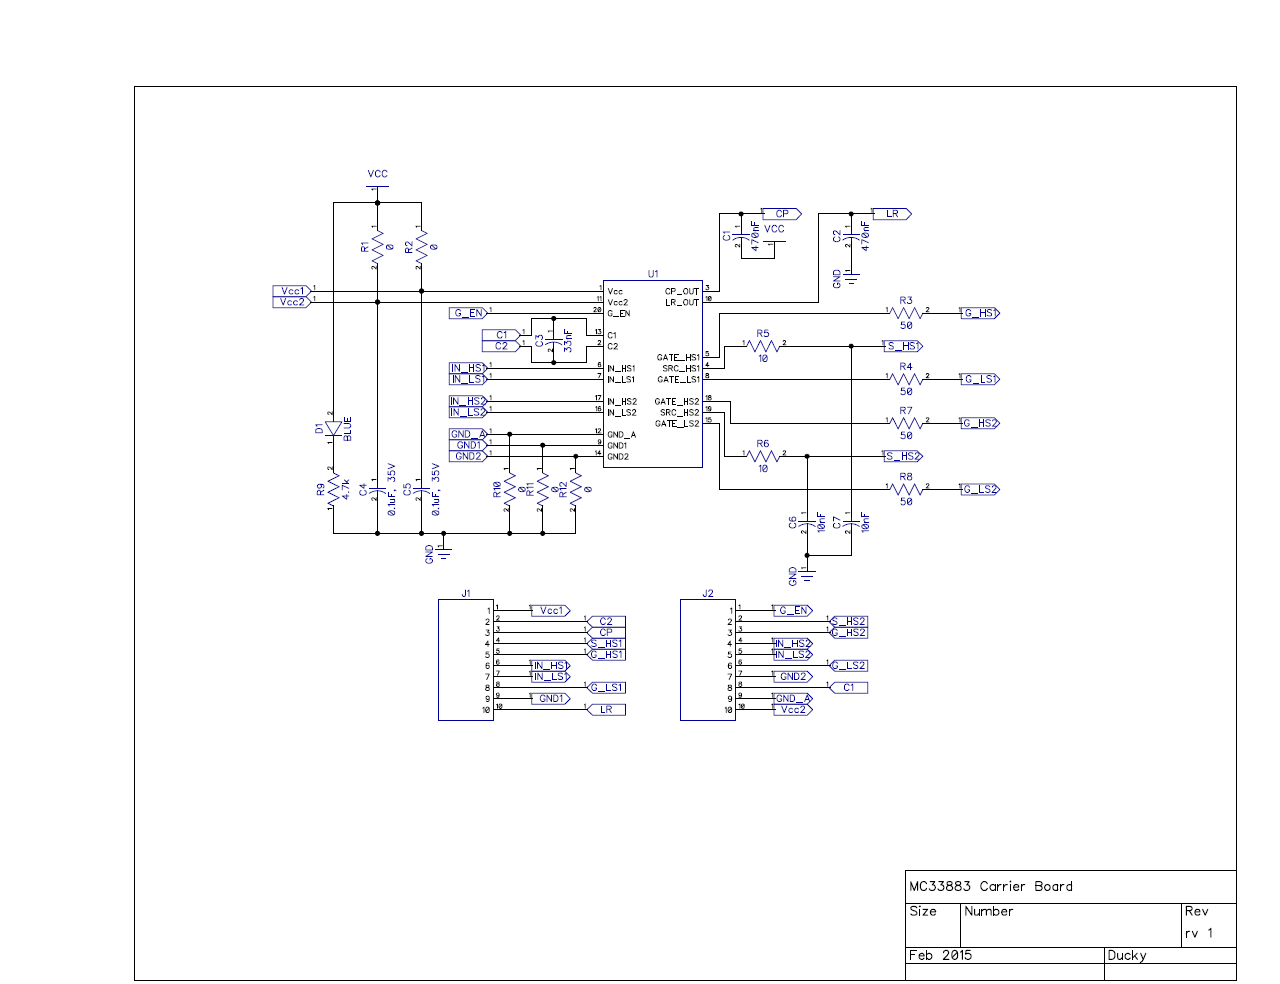
\includegraphics[width=1.0\columnwidth]{images-dis5/mc33883-schematic} \\
  Hopefully a fairly readable schematic
\end{figure}
\end{columns}
\end{frame}

%---------------------------------------------------------------------
\subsection{Advanced Techniques}

% Quadrature encoder
% Gray code for absolute positioning

%---------------------------------------------------------------------
\section{Feedback Control} % [?? mins]
%---------------------------------------------------------------------
\begin{frame}
\centering \huge Feedback Control
\end{frame}

%---------------------------------------------------------------------
\subsection{P control}

%---------------------------------------------------------------------
\subsection{Group Programming & Debugging Exercise}

%---------------------------------------------------------------------
\section{Summary} % [?? mins]

\begin{frame}
\frametitle{Summary}

\end{frame}

\end{document}
